\documentclass[11pt,a4paper]{article}

\usepackage[utf8]{inputenc}
\usepackage[T1]{fontenc}
\usepackage{lmodern}
\usepackage{microtype}
\usepackage[margin=1in]{geometry}
\usepackage{hyperref}
\usepackage{url}
\usepackage{booktabs}
\usepackage{amsfonts}
\usepackage{nicefrac}
\usepackage{xcolor}
\usepackage{graphicx}
\usepackage{amsmath}
\usepackage{array}
\usepackage{multirow}
\usepackage{authblk}
\usepackage{abstract}
\usepackage{titlesec}
\usepackage{parskip}
\usepackage{tikz}
\usepackage{colortbl}
\usetikzlibrary{shapes.geometric, arrows.meta, positioning, fit, backgrounds}

\title{Signal-to-Noise Ratio Detection in Educational Video Content: A Binary Classification Framework Using Transcript Embeddings}

\author{%
  Bidit Das \\
  Independent Researcher \\
  Dallas, Texas, USA \\
  \texttt{biditdas18@gmail.com}
}

\begin{document}

\maketitle

\begin{abstract}
Educational content platforms face a structural misalignment: engagement metrics optimize for
emotional resonance while learners seek informational value. We present a Signal-to-Noise Ratio
(SNR) framework for automated educational content quality assessment applied to YouTube video
transcripts. Our taxonomy defines HIGH signal content as material containing concrete actionable
steps or methodologically sound explanations, and LOW signal content as material dominated by
generic advice, fear-based framing, repetition, or promotional material.

We construct a dataset of 150 real YouTube transcripts (149 received usable ensemble labels;
1 excluded due to simultaneous API failures) and 300 synthetically generated transcripts
spanning three domains: career and self-improvement, technology and artificial intelligence, and
general education. Real transcripts are labeled via a three-model LLM ensemble (GPT-4o mini,
Gemini 2.5 Flash, Llama 3.3 70B) using calibrated domain-specific rubrics, achieving 74\% full
three-model consensus and 82\% average pairwise agreement---a significant improvement over the
53\% pairwise agreement obtained in the initial domain-agnostic setup (which differed in both
rubric and judge ensemble). Labels are treated as
silver quality throughout.

A lightweight binary classifier is trained on 89 real transcripts mixed with 300 synthetic
transcripts and evaluated on a held-out set of 60 real transcripts (89 + 60 = 149 usable real
transcripts total). The best-performing SVM classifier achieves F1~=~0.871 with
recall~=~0.964 on the HIGH signal class (measured against silver labels; this reflects internal
consistency with the labeling pipeline rather than human-validated accuracy), compared to a
majority-class baseline of F1~=~0.000. We demonstrate that domain-specific rubric calibration
and real-data augmentation improve both annotation reliability and classification performance
relative to synthetic-only training baselines (synthetic-only SVM achieves F1~=~0.747 on the
same test set).

All code, datasets, and generation prompts are publicly available at
\url{https://github.com/biditdas18/snr-detector}.
\end{abstract}

\section{Introduction}

The proliferation of educational video content on platforms such as YouTube has created an
information quality problem at scale. While over 500 hours of video are uploaded every minute~\cite{statista_youtube},
platform recommendation algorithms optimize primarily for watch time, click-through rate, and
engagement---metrics that correlate with emotional stimulation rather than informational value.
A fear-mongering video about job loss, a motivational montage of generic advice, or a heavily
promoted course-selling video may outperform a methodologically rigorous tutorial on the same
topic.

This misalignment imposes real costs on learners. Users investing time in low-signal content
receive anxiety without actionability, motivation without method, and promotion without
substance. The problem is particularly acute in high-stakes domains such as career development,
technical skill-building, and immigration decisions, where poor information quality can lead to
consequential decisions based on noise.

We propose a Signal-to-Noise Ratio (SNR) framework that formalizes content quality as a binary
classification task: does this video transcript contain high-quality educational signal? The
binary formulation is intentional. It maps directly to practical deployment scenarios---platform
pre-recommendation filters, user-facing quality badges, and personalized content curation
systems---where a yes/no quality signal is more actionable than a multi-tier rating.

The core challenge is constructing a quality classifier that is (1) grounded in a principled
taxonomy, (2) trained without exhaustive manual annotation, (3) deployable at inference speeds
impractical for frontier LLMs, and (4) honest about its limitations at this stage of development.

This paper makes the following contributions:
\begin{enumerate}
  \item A formal SNR taxonomy for educational video content with explicit criteria for HIGH and
  LOW signal classification.
  \item A scalable dataset construction methodology combining LLM ensemble annotation for real
  transcripts and structured prompt-based generation for synthetic training data.
  \item A lightweight binary classifier using transcript embeddings that approximates LLM
  judgment at a fraction of the inference cost.
  \item A public dataset and codebase enabling reproducibility and community extension.
\end{enumerate}

\section{Related Work}

\textbf{Content Quality Assessment.} Prior work on automated content quality has focused
primarily on news credibility~\cite{rashkin2017}, fact verification~\cite{thorne2018}, and
readability scoring~\cite{pitler2008}. Educational content quality specifically remains
underexplored, with most work addressing either MOOCs with structured curricula or
child-directed content with platform-specific metadata. YouTube educational content presents a
distinct challenge: creator-defined structure, unverified claims, and engagement-optimized
framing exist alongside genuinely high-value instructional material.

\textbf{LLM-as-Judge.} Recent work has established the viability of using large language models
as automated annotators. Zheng et al.~\cite{zheng2023} demonstrate that GPT-4 judgments on
open-ended question answering correlate strongly with human preference, introducing the MT-Bench
benchmark. Fu et al.~\cite{fu2023} show that LLM scoring can be steered toward arbitrary
evaluation dimensions through structured prompting. We build on this paradigm, using a
three-model ensemble to reduce single-model bias.

\textbf{Knowledge Distillation.} Our approach is conceptually related to knowledge
distillation~\cite{hinton2015}, where a lightweight student model is trained to approximate the
behavior of a more capable teacher. Here, the LLM ensemble serves as the teacher, generating
silver labels on real transcripts, while the embedding classifier serves as a deployable student.

\textbf{Sentence Embeddings.} We use sentence-transformer models for transcript
representation~\cite{reimers2019}. These models have demonstrated strong performance on semantic
similarity and classification tasks, and their compact representations enable efficient inference
in resource-constrained deployment settings.

\section{SNR Taxonomy}

We define a binary taxonomy for educational video content quality based on the information value
delivered to a learner per unit of content consumed.

\subsection{HIGH Signal Content}

A transcript is classified as HIGH signal if it satisfies at least two of the following criteria:
\begin{itemize}
  \item \textbf{Methodological coherence:} Ideas build logically on each other. The transcript
  is not a random assembly of disconnected tips.
  \item \textbf{Specificity:} Content includes concrete actionable steps, named frameworks,
  specific statistics, or examples grounded in verifiable reality.
  \item \textbf{Informational novelty:} The transcript provides perspective or knowledge the
  viewer likely did not already possess.
  \item \textbf{Solution orientation:} When addressing problems or risks, the transcript
  provides analysis of causes and suggested next steps, not merely alarming framing.
\end{itemize}

\subsection{LOW Signal Content}

A transcript is classified as LOW signal if it exhibits one or more of the following patterns
at a dominant level ($>$30\% of content):
\begin{itemize}
  \item \textbf{Generic advice:} Vague recommendations without specificity (e.g., ``work hard,''
  ``believe in yourself,'' ``be consistent'') unsupported by method or example.
  \item \textbf{Repetition without progression:} The same point restated in different words with
  no new information added.
  \item \textbf{Fear-based framing:} Emotional urgency or outrage used as the primary hook,
  with no actionable solution offered.
  \item \textbf{Promotional content:} Course selling, channel promotion, or product placement
  dominating the substance.
  \item \textbf{Logical fallacies:} Appeal to authority without evidence, manufactured urgency,
  social pressure, or burden-of-proof shifting.
\end{itemize}

\subsection{Conflict Resolution}

When a transcript contains HIGH-signal content alongside dominant LOW-signal patterns, it is
classified as LOW. This conservative policy reflects deployment intent: a platform filter should
not surface content where significant portions undermine the signal value.

\section{Dataset Construction}

Our dataset comprises three components: a real-transcript evaluation set, a real-transcript
training supplement, and a synthetic training set.

\subsection{Real Transcript Dataset (150 Transcripts)}

We collected 150 YouTube video transcripts across three domains: career and self-improvement,
technology and artificial intelligence, and general education. Transcripts were obtained
programmatically using the \texttt{youtube-transcript-api} library, requiring no manual video
viewing.

Of the 150 collected transcripts, 149 received usable ensemble labels (1 excluded due to
simultaneous API failures from two of three models). These are split into two subsets:
\textbf{Evaluation set} (60 transcripts): Twenty per domain, used exclusively as the held-out
test set. Their labels were committed to GitHub before any model training, providing a
timestamped integrity record. \textbf{Training supplement} (90 collected; 89 retained after the
one exclusion): Thirty per domain collected from established educational channels including IBM
Technology, ByteByteGo, TED-Ed, and CrashCourse. These are mixed with synthetic data during
training to address synthetic-to-real domain shift. The arithmetic 89 + 60 = 149 usable
transcripts is consistent throughout.

\textbf{Rubric Calibration.} Initial annotation using a single domain-agnostic rubric with a
three-model ensemble (GPT-4, Gemini 1.5 Pro, Meta AI) yielded pairwise inter-model agreement of
53\%, approaching the 50\% random baseline for binary classification. We identified two root
causes: (1) content quality criteria are domain-dependent---actionability in career advice
requires procedural steps and timelines, while actionability in general education requires
conceptual clarity rather than action items; and (2) individual models exhibit systematic
labeling biases that a shared rubric cannot resolve.

To address these issues, we developed calibrated domain-specific rubrics through an iterative
multi-agent process. Three judge models (Llama 3.1 8B, Mistral 7B, Qwen 2.5 7B) independently
evaluated each transcript; a coordinator model (Claude Sonnet) diagnosed disagreement patterns
from per-model criterion quotes and proposed targeted rubric revisions. This loop ran until
weighted inter-judge agreement reached convergence or stagnation. The process converged with
final rubrics achieving strong calibration validated against the production labeling ensemble
(see Appendix~\ref{app:rubrics}).

\textbf{LLM Ensemble Annotation.} All 150 transcripts were labeled using a consistent
three-model ensemble: GPT-4o mini (OpenAI), Gemini 2.5 Flash (Google), and Llama 3.3 70B
(Groq), each receiving identical calibrated domain-specific rubrics. This approach follows the
LLM-as-judge paradigm~\cite{zheng2023}, reducing single-model bias through ensemble aggregation.
Final labels were determined by majority vote; one transcript (0.7\%) was excluded due to
simultaneous API failures from two of three models.

The calibrated domain-specific rubrics improved average pairwise inter-model agreement from
53\% (domain-agnostic) to 82\% across domains, with 74\% of transcripts achieving full
three-model consensus. Weighted inter-judge agreement---assigning 1.0 for unanimous consensus
and 0.667 for majority consensus---reached 91\% overall. All labels are treated as silver
quality; human validation is planned as future work.

\textbf{Why LLM Annotation Over Human Annotation.} Human annotation of educational content
quality is subject to two systematic biases that motivated our LLM ensemble design:

Creator bias occurs when annotator familiarity with a channel contaminates content-level
judgment. A viewer who associates a creator with promotional or fear-based content will apply
that reputation to every transcript regardless of what the content actually contains.
Conversely, a viewer who trusts a creator unconditionally may rate low-signal content as HIGH.
In both cases, the label reflects creator identity rather than transcript quality.

Domain bias occurs when annotator interest in a subject inflates or deflates perceived signal.
A software engineer may rate lifestyle advice as inherently noisy regardless of content
structure. A viewer deeply invested in immigration content may rate general geopolitics
discussions as LOW signal by personal preference, not by rubric. Domain bias means that
annotation quality is bounded by the annotator's subject matter coverage---an unacceptable
constraint for a framework intended to generalize across domains.

LLM ensemble annotation mitigates both failure modes. Language model annotation can reduce
creator- and domain-driven human annotator bias, particularly when creator identity is withheld,
producing labels that more closely reflect content structure---though it does not eliminate
model-level bias inherited from pretraining, which is why we treat these labels as silver
quality. This property is particularly valuable for platform-scale deployment, where quality
labels must generalize across creator reputations and viewer demographics.

The evaluation set contains 28 HIGH (47\%) and 32 LOW (53\%) transcripts. Table~\ref{tab:eval}
shows the evaluation set distribution by domain.

\begin{table}[h]
\centering
\caption{Real Transcript Evaluation Set Distribution (n=60)}
\label{tab:eval}
\begin{tabular}{lccc}
\toprule
Domain & HIGH & LOW & Total \\
\midrule
Career \& Self-Improvement & 4 & 16 & 20 \\
Technology \& AI & 7 & 13 & 20 \\
General Education & 17 & 3 & 20 \\
\midrule
Total & 28 & 32 & 60 \\
\bottomrule
\end{tabular}
\end{table}

\subsection{Synthetic Training Set}

To enable balanced classifier training without manual annotation, we generated 300 synthetic
transcripts using the Anthropic Claude API. Each transcript was generated using a structured
domain-specific prompt explicitly designed to elicit either HIGH or LOW signal content (see
Appendix~\ref{app:synthetic} for full prompt templates).

Labels for synthetic transcripts are assigned by construction: a transcript generated by a
HIGH-signal prompt is labeled HIGH by definition. This removes manual annotation ambiguity for the synthetic subset, though it does not guarantee
that every generated transcript perfectly satisfies its intended class definition---prompt-adherence
errors remain possible. We therefore treat synthetic labels as high-confidence but not error-free.

The synthetic training set comprises 150 HIGH and 150 LOW transcripts distributed equally
across the three domains (50 HIGH + 50 LOW per domain), yielding a balanced training set that
mitigates class imbalance during learning. Synthetic transcripts target 400--500 words to
approximate the length distribution of real transcripts in our evaluation set.

\begin{table}[h]
\centering
\caption{Synthetic Training Set Distribution}
\label{tab:synthetic}
\begin{tabular}{lccc}
\toprule
Domain & HIGH & LOW & Total \\
\midrule
Career \& Self-Improvement & 50 & 50 & 100 \\
Technology \& AI & 50 & 50 & 100 \\
General Education & 50 & 50 & 100 \\
\midrule
Total & 150 & 150 & 300 \\
\bottomrule
\end{tabular}
\end{table}

\subsection{Dataset Integrity Protocol}

All label files (\texttt{test\_set\_final.csv}, \texttt{train\_set\_final.csv},
\texttt{all\_150\_silver\_labels.csv}) and result artifacts are version-controlled in a public
GitHub repository, providing an immutable, publicly auditable record. Labels were not modified
after publication. Synthetic transcript labels are deterministic by construction and fully
reproducible from the published generation prompts.

\section{Methodology}

Figure~\ref{fig:arch} illustrates the full SNR-Detect system. The annotation pipeline (top)
runs offline to produce silver labels; the classification pipeline (bottom) runs at inference
on any YouTube transcript.

\begin{figure}[ht]
\centering
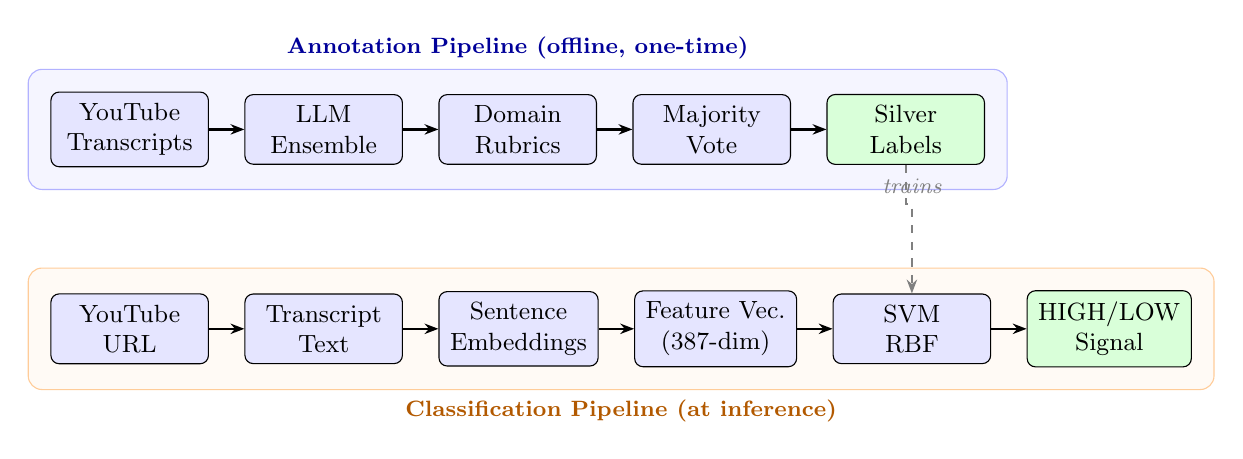
\begin{tikzpicture}[
  box/.style={rectangle, rounded corners=3pt, draw=black, fill=blue!10,
              align=center, minimum height=0.7cm, minimum width=2.0cm,
              font=\small, inner sep=4pt},
  outbox/.style={rectangle, rounded corners=3pt, draw=black, fill=green!15,
              align=center, minimum height=0.7cm, minimum width=2.0cm,
              font=\small, inner sep=4pt},
  arr/.style={-{Stealth[length=5pt]}, thick},
  darr/.style={-{Stealth[length=5pt]}, thick, dashed, gray},
  lbl/.style={font=\small\itshape, text=gray!70!black, align=right}
]

\node[box] (yt)   {YouTube\\Transcripts};
\node[box, right=0.45cm of yt]  (llm)  {LLM\\Ensemble};
\node[box, right=0.45cm of llm] (rub)  {Domain\\Rubrics};
\node[box, right=0.45cm of rub] (mv)   {Majority\\Vote};
\node[outbox, right=0.45cm of mv]  (sl)   {Silver\\Labels};

\draw[arr] (yt)  -- (llm);
\draw[arr] (llm) -- (rub);
\draw[arr] (rub) -- (mv);
\draw[arr] (mv)  -- (sl);

\node[box, below=1.6cm of yt]   (url)  {YouTube\\URL};
\node[box, right=0.45cm of url] (txt)  {Transcript\\Text};
\node[box, right=0.45cm of txt] (emb)  {Sentence\\Embeddings};
\node[box, right=0.45cm of emb] (fv)   {Feature Vec.\\(387-dim)};
\node[box, right=0.45cm of fv]  (svm)  {SVM\\RBF};
\node[outbox, right=0.45cm of svm] (out) {HIGH/LOW\\Signal};

\draw[arr] (url) -- (txt);
\draw[arr] (txt) -- (emb);
\draw[arr] (emb) -- (fv);
\draw[arr] (fv)  -- (svm);
\draw[arr] (svm) -- (out);

\draw[darr] (sl.south) -- ++(0,-0.5) -| (svm.north)
  node[midway, above, font=\footnotesize\itshape, text=gray] {trains};

\begin{scope}[on background layer]
  \node[draw=blue!30, fill=blue!4, rounded corners=5pt, inner sep=8pt,
        fit=(yt)(sl), label={[font=\footnotesize\bfseries, text=blue!60!black]above:Annotation Pipeline (offline, one-time)}] {};
  \node[draw=orange!40, fill=orange!4, rounded corners=5pt, inner sep=8pt,
        fit=(url)(out), label={[font=\footnotesize\bfseries, text=orange!70!black]below:Classification Pipeline (at inference)}] {};
\end{scope}

\end{tikzpicture}
\caption{SNR-Detect system architecture. \textit{Top:} The annotation pipeline labels real
transcripts offline using a three-model LLM ensemble with calibrated domain-specific rubrics.
\textit{Bottom:} The classification pipeline embeds any YouTube transcript into a 387-dimensional
feature vector (384 sentence embedding + 3 domain one-hot) and classifies it as HIGH or LOW
signal using a trained SVM classifier. The dashed arrow indicates that silver labels from the
annotation pipeline are used to train the classifier.}
\label{fig:arch}
\end{figure}

\subsection{Task Formulation}

We formulate SNR classification as binary: given a YouTube video transcript $t$, predict
$y \in \{\text{HIGH}, \text{LOW}\}$. HIGH indicates content worth watching for its educational
value; LOW indicates content that fails to deliver meaningful signal relative to time invested.

\subsection{Transcript Representation}

We represent transcripts as dense semantic embeddings using the \texttt{all-MiniLM-L6-v2}
sentence-transformer model~\cite{reimers2019}, mapping variable-length transcript text to fixed
384-dimensional vectors. To provide domain context without splitting the classifier, we
concatenate a three-dimensional one-hot domain encoding, yielding a 387-dimensional feature
vector per transcript. This allows the classifier to learn domain-specific decision boundaries
within a single unified model while preserving the full training dataset size.

Embeddings are computed independently for training and test transcripts, with no information
leakage between splits.

\subsection{Classifiers}

We train two binary classifiers on the mixed training set:
\begin{itemize}
  \item \textbf{Logistic Regression (LR):} L2 regularization, $C{=}1.0$,
  \texttt{class\_weight='balanced'}, trained to convergence (\texttt{max\_iter=1000}).
  \item \textbf{Support Vector Machine (SVM):} RBF kernel, $C{=}1.0$,
  \texttt{class\_weight='balanced'}, selected for effectiveness in high-dimensional embedding
  spaces~\cite{cortes1995}.
\end{itemize}

Both classifiers are trained on a mixed set of 389 transcripts (89 real silver-labeled + 300
balanced synthetic) and evaluated on the 60 held-out real transcripts. The mixed training set
directly exposes the classifier to real YouTube content distributions during training, addressing
the synthetic-to-real domain shift observed in synthetic-only baselines.

\subsection{Baseline}

We compare against a majority-class baseline that predicts LOW for every transcript. This
baseline represents the trivially achievable performance ceiling for a zero-information
classifier and demonstrates that accuracy alone is insufficient for evaluating imbalanced
classification tasks~\cite{hegarcia2009}.

\subsection{Evaluation Protocol}

We evaluate on the 60-transcript real silver-labeled test set using:
\begin{itemize}
  \item \textbf{Accuracy:} overall classification rate
  \item \textbf{F1 (HIGH class):} primary metric given class imbalance; harmonic mean of
  precision and recall for the minority HIGH class
  \item \textbf{Precision and Recall:} breakdown of HIGH-class performance
  \item \textbf{Confusion matrix:} full outcome breakdown
\end{itemize}

F1 on the HIGH class is the primary metric, as it captures the classifier's ability to identify
genuine educational signal. The calibrated domain-specific rubric produced a more balanced test
set (47\% HIGH, 53\% LOW) than initial annotation (20\% HIGH), reflecting the rubric's improved
ability to distinguish genuinely high-signal content from borderline cases.

\section{Results}

\subsection{Classification Performance}

Table~\ref{tab:results} presents classification results on the 60-transcript held-out evaluation
set.

\begin{table}[h]
\centering
\caption{Classification Results on Real Transcript Test Set (n=60)}
\label{tab:results}
\begin{tabular}{lcccc}
\toprule
Model & Acc. & F1 & Prec. & Rec. \\
\midrule
Baseline (majority LOW) & 0.533 & 0.000 & 0.000 & 0.000 \\
\midrule
\multicolumn{5}{l}{\textit{Synthetic-only training (300 synthetic transcripts; matched test set)}} \\
SVM RBF (synth-only, thresh=0.50) & 0.683 & 0.747 & 0.596 & 1.000 \\
Log.\ Regression (synth-only, thresh=0.50) & 0.683 & 0.732 & 0.605 & 0.929 \\
\midrule
\multicolumn{5}{l}{\textit{Mixed training (89 real + 300 synthetic; 389 total)}} \\
Log.\ Regression (thresh=0.55) & 0.850 & 0.857 & 0.771 & 0.964 \\
SVM RBF (thresh=0.50) & 0.867 & 0.871 & 0.794 & 0.964 \\
\bottomrule
\end{tabular}
\end{table}

The SVM classifier achieves F1~=~0.871 on the HIGH signal class, identifying 96.4\% of genuine
HIGH signal transcripts (recall~=~0.964). The majority-class baseline achieves only 0.533
accuracy---confirming that the calibrated rubric produced a near-balanced test set and that
accuracy alone is an insufficient metric for this task. The trained classifier provides strong
discriminative signal where the baseline provides none.

The high recall (0.964) reflects a deliberate threshold choice appropriate for content
filtering: surfacing a false positive (mislabeled LOW as HIGH) is preferable to missing genuine
educational signal. Table~\ref{tab:results} shows directly comparable synthetic-only baselines
trained and evaluated on the same splits. The mixed-training SVM improves F1 from 0.747
(synthetic-only) to 0.871 and precision from 0.596 to 0.794, demonstrating that mixing 89 real
transcripts into training substantially reduces the false positive rate by exposing the
classifier to authentic YouTube content distributions during learning.

\subsection{Domain Feature Ablation}

To assess whether the classifier exploits domain priors encoded in the 3-dimensional one-hot
domain feature, we trained an SVM-RBF on the full mixed training set using 384-dimensional
sentence embeddings only (no domain one-hot). The no-domain SVM achieves F1~=~0.844,
accuracy~=~0.833, precision~=~0.750, and recall~=~0.964 on the held-out test set (results
saved to \texttt{reports/ablation\_no\_domain.json}). The modest F1 reduction of 0.027 relative
to the full 387-dimensional model (F1~=~0.871) suggests the domain feature provides marginal
discriminative value beyond what the semantic embedding already captures, and that the
classifier is not primarily exploiting domain-level class imbalance.

\subsection{Annotation Reliability}

The calibrated domain-specific rubrics improved average pairwise inter-model agreement from
53\% (initial domain-agnostic rubric) to 82\% across career and general education domains,
with the technology/AI domain achieving 95\% pairwise agreement between GPT-4o mini and Gemini
2.5 Flash. Weighted inter-judge agreement reached 91\% overall (74\% full three-model
consensus). Because the initial (53\%) and production (82\%) settings differ in both the rubric and the
judge ensemble (GPT-4 / Gemini 1.5 Pro / Meta AI vs.\ GPT-4o mini / Gemini 2.5 Flash /
Llama 3.3 70B), this improvement reflects their combined effect; isolating the causal
contribution of rubric calibration alone would require holding the judge ensemble fixed across
both rubrics. The 82\% figure refers to the production frontier ensemble; the local calibration
panel reported in the companion paper converged on two of three domains, with the Career domain
remaining below target.

The test set labels were assigned by the same class of frontier LLM models used to label the
training supplement, which may introduce correlated label bias. Human validation remains planned
future work.

\subsection{Confusion Matrix}

Figure~\ref{fig:cm} presents the confusion matrix for the best-performing classifier (SVM RBF,
threshold~=~0.50) on the held-out test set.

\begin{figure}[ht]
\centering
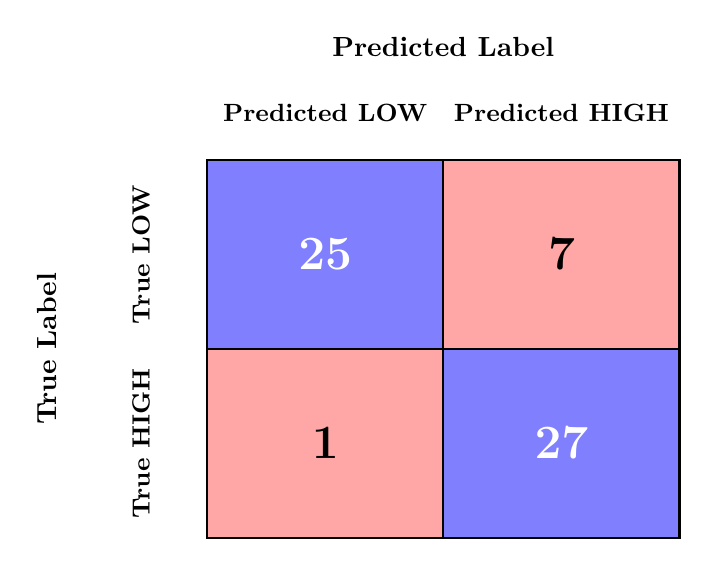
\begin{tikzpicture}[font=\normalsize, scale=1.2]

  \fill[blue!50]  (2,2) rectangle (4.5,4);
  \node[font=\LARGE\bfseries, text=white] at (3.25, 3.0) {25};

  \fill[red!35]   (4.5,2) rectangle (7,4);
  \node[font=\LARGE\bfseries]             at (5.75, 3.0) {7};

  \fill[red!35]   (2,0) rectangle (4.5,2);
  \node[font=\LARGE\bfseries]             at (3.25, 1.0) {1};

  \fill[blue!50]  (4.5,0) rectangle (7,2);
  \node[font=\LARGE\bfseries, text=white] at (5.75, 1.0) {27};

  \draw[thick] (2,0) rectangle (7,4);
  \draw[thick] (4.5,0) -- (4.5,4);
  \draw[thick] (2,2)   -- (7,2);

  \node[font=\small\bfseries] at (3.25, 4.5) {Predicted LOW};
  \node[font=\small\bfseries] at (5.75, 4.5) {Predicted HIGH};
  \node[font=\normalsize\bfseries] at (4.5, 5.2) {Predicted Label};

  \node[font=\small\bfseries, rotate=90] at (1.3, 3.0) {True LOW};
  \node[font=\small\bfseries, rotate=90] at (1.3, 1.0) {True HIGH};
  \node[font=\normalsize\bfseries, rotate=90] at (0.3, 2.0) {True Label};

\end{tikzpicture}
\caption{Confusion matrix on the 60-transcript held-out test set (SVM RBF, threshold~=~0.50).
Rows indicate true labels; columns indicate predicted labels. Train set: 89 real + 300 synthetic
transcripts. The classifier achieves recall~=~0.964 on the HIGH signal class.}
\label{fig:cm}
\end{figure}

\subsection{Error Analysis}

We inspected misclassified transcripts to characterize systematic failure modes. Two residual
patterns emerged:

\begin{itemize}
  \item \textbf{Motivational framing with embedded specifics:} Transcripts containing genuine
  actionable content but opening with emotional hooks that activate LOW-signal features in
  embedding space. Career self-improvement content is particularly susceptible, as motivational
  language and procedural steps co-occur more frequently in this domain.
  \item \textbf{Boundary ambiguity:} Transcripts with roughly equal proportions of HIGH and LOW
  signal content present irreducible classification difficulty. The 82\% average pairwise
  inter-model agreement confirms that human-like boundary cases are not unique to the
  classifier---even frontier LLMs disagree on these examples.
\end{itemize}

\section{Limitations}

\textbf{Silver label quality.} All labels in this work are silver quality, assigned by LLM
ensemble majority vote following calibrated domain-specific rubrics. While inter-model agreement
improved substantially from 53\% (domain-agnostic) to 82\% average pairwise (domain-specific),
LLM judges may reflect systematic biases inherited from pretraining. The test set labels were
produced by the same class of frontier LLM models used to label the training supplement, which
may introduce correlated label bias. Human validation via crowdsourced annotation with Cohen's
$\kappa$ computation is planned as immediate future work.

\textbf{Real training data concentration.} The 89 real training transcripts were collected
predominantly from established educational channels (IBM Technology, ByteByteGo, TED-Ed,
CrashCourse), which skew toward HIGH signal content. LOW signal representation in training is
primarily provided by synthetic transcripts, which may not fully capture naturalistic LOW signal
patterns.

\textbf{YouTube scope.} This study is scoped exclusively to YouTube transcripts. The SNR
framework may not transfer without adaptation to shorter-form content (e.g., Instagram Reels,
TikTok) where transcript length and narrative structure differ substantially.

\textbf{Narrow domain coverage.} Three domains were selected for this pilot study.
Generalization to medical, legal, and financial educational content requires additional
validation given the higher stakes of quality errors in those domains.

\textbf{Small real test set.} The evaluation set contains 60 transcripts (n=60), limiting the
statistical reliability of reported metrics. Given the small test set, we report 95\% Wilson
score intervals for the rate-based metrics, computed from the confusion matrix: accuracy 0.867
[0.758, 0.931], recall 0.964 [0.823, 0.994], precision 0.794 [0.632, 0.897]. These wide
intervals underscore that all reported metrics are feasibility-stage estimates rather than stable
performance claims; a bootstrap interval for F1 and larger-scale validation are scoped to future
work. This paper positions itself as a feasibility study and framework contribution.

\section{Future Work}

\textbf{Human validation.} We will recruit independent annotators via Prolific to label a
transcript subset, enabling computation of human-LLM agreement (Cohen's $\kappa$) as a more
reliable evaluation benchmark. Annotators will be selected across domains to measure whether
domain bias affects human label quality relative to the LLM ensemble baseline.

\textbf{Two-Mode Deployment Architecture.} We envision two distinct deployment modes with
fundamentally different bias profiles:

Personal deployment treats annotator bias as a feature rather than a flaw. A user's domain
preferences and creator associations are valid personal signal. A personal SNR tool learns from
individual feedback, surfacing content that matches the user's definition of educational value
and warning against content that matches their historical noise patterns. Human bias is
intentionally preserved and personalized.

Platform deployment requires the opposite approach. A recommendation filter must generalize
across millions of viewers with heterogeneous domain preferences and creator associations. Here,
LLM ensemble annotation---and eventually, majority consensus from large-scale user
feedback---washes out individual bias. Platform-scale labels reflect population-level signal
quality, not any single annotator's preferences. Existing ``was this helpful'' user signals from
platforms such as YouTube represent an untapped training signal for this mode.

This two-mode architecture cleanly separates the bias question: personal tools embrace it,
platform tools reduce it. Both are valid applications of the SNR framework with different
annotation strategies.

\textbf{Personalized quality learning.} A user-facing deployment can collect binary helpfulness
feedback and periodically fine-tune a personal SNR classifier. Population Stability Index
monitoring~\cite{yurdakul2018} detects preference drift and triggers model refresh, enabling
adaptation as user educational interests evolve.

\textbf{Domain expansion.} Future dataset collection will extend to medical, legal, and
financial educational content, where signal-to-noise distinction carries higher consequential
stakes.

\section{Conclusion}

We presented SNR-Detect, a binary classification framework for educational video content quality
assessment. Our SNR taxonomy formalizes the distinction between content that delivers genuine
educational value and content dominated by noise patterns---a distinction that existing platform
metrics fail to capture. We showed that moving to domain-specific rubrics together with the production labeling ensemble
raised pairwise inter-model agreement from 53\% to 82\%, and that mixing real
transcripts into classifier training improves performance, achieving F1~=~0.871 (measured
against silver labels; reflecting internal consistency with the labeling pipeline rather than
human-validated accuracy) with recall~=~0.964 on the HIGH signal class---compared to F1~=~0.747
for a synthetic-only baseline evaluated on the same test set.

The key contributions are methodological: a reproducible pipeline for dataset construction
without exhaustive manual annotation, a domain-specific rubric calibration procedure that
substantially improves LLM ensemble annotation reliability, and a deployable classifier that
approximates LLM judgment at a fraction of the inference cost. The framework lays groundwork for
platform-level content filtering and personalized quality learning systems where real-time,
low-cost inference is a hard requirement.

We release all code, datasets, and generation prompts at
\url{https://github.com/biditdas18/snr-detector}.

\begin{thebibliography}{10}

\bibitem{rashkin2017}
Hannah Rashkin, Eunsol Choi, Jin Yea Jang, Svitlana Volkova, and Yejin Choi.
\newblock Truth of varying shades: Analyzing language in fake news and political fact-checking.
\newblock In {\em Proceedings of the 2017 Conference on Empirical Methods in Natural Language Processing}, pages 2931--2937, 2017.

\bibitem{thorne2018}
James Thorne, Andreas Vlachos, Christos Christodoulopoulos, and Arpit Mittal.
\newblock {FEVER}: A large-scale dataset for fact extraction and {VERification}.
\newblock In {\em Proceedings of the 2018 Conference of the North American Chapter of the Association for Computational Linguistics}, pages 809--819, 2018.

\bibitem{pitler2008}
Emily Pitler and Ani Nenkova.
\newblock Revisiting readability: A unified framework for predicting text quality.
\newblock In {\em Proceedings of the 2008 Conference on Empirical Methods in Natural Language Processing}, pages 186--195, 2008.

\bibitem{zheng2023}
Lianmin Zheng, Wei-Lin Chiang, Ying Sheng, Siyuan Zhuang, Zhanghao Wu, Yonghao Zhuang, Zi Lin, Zhuohan Li, Dacheng Li, Eric~P. Xing, Hao Zhang, Joseph~E. Gonzalez, and Ion Stoica.
\newblock Judging {LLM}-as-a-judge with {MT}-bench and chatbot arena.
\newblock In {\em Advances in Neural Information Processing Systems}, volume~36, 2023.

\bibitem{fu2023}
Jinlan Fu, See-Kiong Ng, Zhengbao Jiang, and Pengfei Liu.
\newblock {GPTScore}: Evaluate as you desire.
\newblock {\em arXiv preprint arXiv:2302.04166}, 2023.

\bibitem{hinton2015}
Geoffrey Hinton, Oriol Vinyals, and Jeff Dean.
\newblock Distilling the knowledge in a neural network.
\newblock {\em arXiv preprint arXiv:1503.02531}, 2015.

\bibitem{reimers2019}
Nils Reimers and Iryna Gurevych.
\newblock Sentence-{BERT}: Sentence embeddings using siamese {BERT}-networks.
\newblock In {\em Proceedings of the 2019 Conference on Empirical Methods in Natural Language Processing}, pages 3982--3992, 2019.

\bibitem{cortes1995}
Corinna Cortes and Vladimir Vapnik.
\newblock Support-vector networks.
\newblock {\em Machine Learning}, 20(3):273--297, 1995.

\bibitem{hegarcia2009}
Haibo He and Edwardo A. Garcia.
\newblock Learning from imbalanced data.
\newblock {\em IEEE Transactions on Knowledge and Data Engineering}, 21(9):1263--1284, 2009.

\bibitem{yurdakul2018}
Bilal Yurdakul and Joshua D. Naranjo.
\newblock Statistical properties of the population stability index.
\newblock {\em Journal of Risk Model Validation}, 2019.

\bibitem{statista_youtube}
Statista.
\newblock Hours of video uploaded to YouTube every minute.
\newblock \url{https://www.statista.com/statistics/259477/hours-of-video-uploaded-to-youtube-every-minute/}, accessed June 2026.

\end{thebibliography}

\appendix

\section{Calibrated Domain-Specific Rubrics}
\label{app:rubrics}

The following calibrated rubrics were used for all 150 real transcript labels. Each domain
received a separate rubric following iterative multi-agent calibration. All three annotators
(GPT-4o mini, Gemini 2.5 Flash, Llama 3.3 70B) received identical domain-specific rubrics.

\textbf{Career \& Self-Improvement --- HIGH SIGNAL} requires at least 2 of: (1) Specific
procedural steps with named methods, tools, timelines, or defined techniques; (2) Concrete
outcomes or metrics---numbers, percentages, named frameworks; (3) Specific action plan or named
solution when addressing a problem; (4) Sequential ideas where each point adds new information.

\textbf{Career \& Self-Improvement --- LOW SIGNAL} (any one dominant): (1) Motivational
language dominates with no actionable method---phrases like ``believe in yourself'' appear
repeatedly and procedural steps are absent; (2) Same warning or point repeated more than twice;
(3) Primary hook is fear or urgency with no concrete mitigation; (4) More than 30\% promotes a
course, service, or product; (5) Claims are authoritative but cite no evidence---named books,
frameworks, or cited statistics do NOT trigger this criterion.

\textbf{Technology \& AI --- HIGH SIGNAL} requires at least 2 of: (1) Named technologies,
algorithms, or architectural patterns with accurate technical detail; (2) Mechanism or tradeoff
explained---not just what but why; (3) Concrete and implementable code concepts, benchmarks, or
design decisions; (4) Specific solution path for a technical problem.

\textbf{Technology \& AI --- LOW SIGNAL} (any one dominant): (1) Hype language without
technical substance; (2) Sweeping unsubstantiated claims about AI capabilities or job market;
(3) Primary message is fear with no actionable technical skill; (4) Technology recommended
without explaining what it does or why; (5) More than 30\% promotes a paid resource---a brief
sponsor mention alone does NOT qualify.

\textbf{General Education --- HIGH SIGNAL} requires at least 2 of: (1) Mechanism or concept
explained from first principles with logical steps; (2) Specific analogy, thought experiment,
or concrete example that illuminates the concept accurately; (3) Non-obvious insight or
counterintuitive conclusion; (4) Accurate representation of complexity; (5) Historical context,
causal analysis, or named expert perspectives when covering problems.

\textbf{General Education --- LOW SIGNAL} (any one dominant): (1) Alarming or conspiratorial
framing as primary hook without evidence; (2) Confident causal claims without evidence or
logical reasoning; (3) Complex phenomena presented as simple good-vs-evil narratives; (4)
Emotional manipulation dominates over explanation. Note: absence of actionable steps does NOT
indicate LOW signal for general education.

\textbf{Conflict rule (all domains):} If HIGH-signal content coexists with dominant LOW-signal
patterns ($>$30\% of transcript), assign LOW.

\section{Synthetic Training Transcripts}
\label{app:synthetic}

The 300 synthetic transcripts used for classifier training are available in the project
repository at: \url{https://github.com/biditdas18/snr-detector/blob/main/data/synthetic/synthetic_transcripts.csv}

Each transcript includes domain, signal level (HIGH/LOW), and generated text. Labels are
assigned by construction from the generation prompt---HIGH prompts produce HIGH transcripts by
definition.

\end{document}
